\chapter{Эксперименты}

Эксперименты проводятся в мультиагентной среде multiagent-particle-envs \cite{multiagent-particle-envs} от компании OpenAI.


\section{Сценарий 1. Simple Speaker Listener}  \label{ch4:exp-ssl}

Сценарий \textit{Simple Speaker Listener} воспроизводится и тестируется с использованием алгоритма MADDPG \cite{lowe2017multiagent}.

Сценарий упоминается в разделе \hyperref[intro:ssl]{0.2.1}. В этом сценарии два агента имеют разные пространства действий и наблюдений. Наблюдение \textit{говоруна} $o_s$ - это цвет цели, обозначенный 3- канальным вектором $d \in \mathbb{R}^3$. Наблюдение \textit{слушателя} $o_l$ – это вектор конкатенации его собственной скорости $\upsilon \in \mathbb{R}^2$ его расстояния до трех ориентиров $p = [p_1, p_2, p_3], p_i \in \mathbb{R}^2$ и сигнал, произнесенный \textit{говоруном} на предыдущем временном шаге. Это:

\begin{equation}
    \begin{multlined}
        o_s = [d]
        o_l = [\upsilon, p, c]
    \end{multlined}
\end{equation}

Коммуникационное действие \textit{говоруна} обозначается «one-hot encoding» вектором $[1; 0; 0]$ или $[0; 1; 0]$ или $[0; 0; 1]$, для обозначения трех ориентиров соответственно.
Физическое действие \textit{u} слушателя - это 5-канальный вектор, каждый из которых представляет одно направление движения (вверх, вниз, влево, вправо или без движения). Наблюдения и действия \textit{говоруна} и \textit{слушателя} и их взаимосвязь показаны на рисунке \firef{fig:ch4-ssl}.

\begin{figure}[ht!]
    \center
    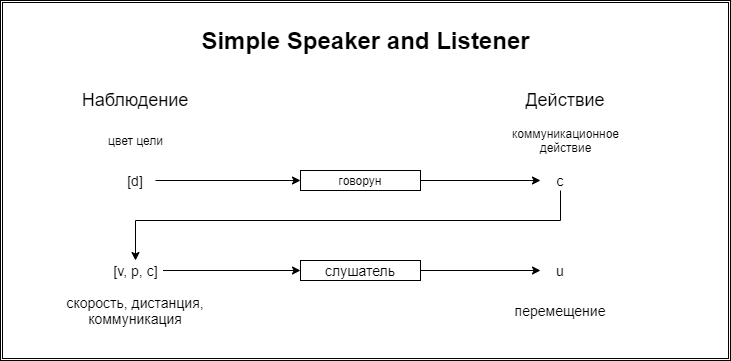
\includegraphics [scale=0.60] {my_folder/images/ch4/simple_speaker_listener.png}
    \caption{\textit{Говорун} наблюдает цвет целевого ориентира \textit{d} и издает коммуникационое действие, которое будет получено \textit{слушателем}. \textit{Слушатель} производит физическое движение.}
    \label{fig:ch4-ssl}
\end{figure}

Два агента имеют общую награду \textit{r}, которая является отрицательным евклидовым расстоянием между \textit{слушателем} и его целью. Проблема, которую необходимо решить в этом сценарии, заключается в поиске оптимальных политик для \textit{говоруна} и \textit{слушателя}, чтобы максимизировать ожидаемую награду, то есть $\max_{\pi}R(\pi)$, где

\begin{equation}
    \begin{multlined}
        R(\pi) = \mathbb{E}[\sum_{t=0}^{T}r(s_t, a_t)]
    \end{multlined}
\end{equation}

Во время обучения \textit{говорун} учится различать три ориентира и передавать целевой ориентир \textit{слушателю}. И \textit{слушатель} должен изучить закодированные высказывания, говоруна, и перейти к правильной цели.

TODO: уточнить параметры

Архитектура актор-сети \textit{говоруна} аналогична архитектуре \textit{слушателя}, каждый из которых содержит два полно связанных слоя с 64 нейронами и использует функцию активации relu. Однако их выходные слои различаются с точки зрения количества единиц и функций активации. Для \textit{говоруна} используется функция активации Gumbel-Softmax, а для слушателя - tanh. Сети критиков имеют структуру, аналогичную сетям акторов, за исключением того, что они выдают скалярное Q-значение.


\section{Сценарий 2}

TODO


\section{Сценарий 3}

TODO

\newpage
